\documentclass[jou,a4paper]{apa6}
\usepackage{enumitem}
\usepackage{fancyhdr}
\pagestyle{fancy}
\setlength{\headheight}{25pt}
\usepackage[breaklinks=True]{hyperref}
\usepackage{url}
\usepackage{lastpage}
\usepackage[natbibapa]{apacite} 
\bibliographystyle{apacite}
\usepackage{amsmath} % to split equation across lines

\begin{document}

% JEMR Definitions
\newcommand{\jemrVolume}{x}
\newcommand{\jemrIssue}{y}
\newcommand{\jemrArticle}{z}
\newcommand{\jemrLastPage}{\pageref{LastPage}}
\newcommand{\jemrReceivedDate}{Mmm dd, 2016}
\newcommand{\jemrPublishedDate}{Mmm dd, 2016}
\newcommand{\jemrShortTitle}{``Ocular tremor'' in Parkinson's disease}
% JEMR-specific definitions

\setlist[itemize]{noitemsep, topsep=0pt}

\makeatletter
\renewcommand*{\addperi}[1]{#1.~}

\renewcommand{\section}{\@startsection {section}{1}{24pt}%
{12pt}{12pt}%
{\centering\normalfont\large}}

\renewcommand{\subsection}{\@startsection{subsection}{2}{0pt}%
{6pt}{6pt}%
{\normalfont\normalsize\itshape}}

\renewcommand{\subsubsection}{\@startsection{subsubsection}{3}{24pt}%
{\parskip}%
{-\parskip}%
{\normalfont\normalsize\itshape\bfseries\addperi}}

\makeatother

% header on first page
\fancypagestyle{plain}{%
\fancyhf{} % clear all header and footer fields
\fancyhead[L]{\small
Journal of Eye Movement Research\\
\jemrVolume(\jemrIssue):\jemrArticle, 1-\jemrLastPage}
\fancyfoot[C]{\thepage}
\renewcommand{\headrulewidth}{0pt}
\renewcommand{\footrulewidth}{0pt}}

% End of JEMR Definitions

\title{``Pervasive ocular tremor of Parkinson's'' is not pervasive, ocular, or uniquely parkinsonian.}
\fiveauthors
	{Michael R. MacAskill}
	{Daniel J. Myall}
	{Toni L. Pitcher}
	{Masayuki Watanabe}
	{Tim J. Anderson}
\fiveaffiliations
    {New Zealand Brain Research Institute,\\Christchurch\\
    Department of Medicine, University of Otago, Christchurch}
    {New Zealand Brain Research Institute,\\Christchurch}
    {New Zealand Brain Research Institute,\\Christchurch\\
    Department of Medicine, University of Otago, Christchurch}
	{New Zealand Brain Research Institute,\\Christchurch}
    {New Zealand Brain Research Institute,\\Christchurch\\
    Department of Medicine, University of Otago, Christchurch\\
    Department of Neurology, Christchurch Hospital\\
    Brain Research New Zealand (Rangahau Roro Aotearoa)}

\abstract{
A putative tremulous oscillation of the eyes has been proposed to provide the long-sought objective, sensitive and specific diagnostic sign for Parkinson's disease . Vigorous debate has ensued as to whether this ``ocular tremor'' is a real phenomenon or an artefact secondary to head motion. Contradictory arguments have centred on the capabilities of magnetic movement measurement technologies, with small numbers of illustrative cases presented to bolster either side. A large, definitive study able to either confirm or reject the original finding on a purely oculographic basis was required.
We examined 681 oculomotor recordings from a longitudinal study of 188 Parkinson's patients and 66 controls. Fourier analysis was used to detect oscillations not only in their raw pupil motion data but also in corneal reflection signals, which can correct for head motion.
We replicated the original authors' findings inasmuch as we detected oscillations in raw pupil position data that often occurred in their reported frequency range of 5.7 $\pm$ 3 Hz. They were not, however, present universally in patients and the frequency (if not power) distribution was similar in controls. Crucially, oscillations in that frequency range were abolished when corneal reflection correction was applied to compensate for head-motion. The oscillations in the uncorrected data were strongly related to clinical ratings of somatomotor tremor severity. We found strong evidence that the postulated purely ocular tremor of Parkinson's does not exist, other than as an artefact arising from head motion secondary to somatic tremor.
\\
\noindent\rule[0.5ex]{\linewidth}{1pt}
\\
{\bf Keywords: eye movement, eye tracking, gaze, pupil-centre corneal-reflex video-oculography, Parkinson's disease, tremor, head motion}}

\shorttitle{Manuscript Submission}
\rightheader{}
\leftheader{}

\maketitle

\lhead{
Journal of Eye Movement Research\\
\jemrVolume(\jemrIssue):\jemrArticle, 1--\jemrLastPage
}
\rhead{
MacAskill, Myall, Pitcher, Watanabe, \& Anderson (2016)\\
\jemrShortTitle
}
\thispagestyle{plain}

\begin{figure}[!b]
  \fbox{
  \begin{minipage}{0.455\textwidth}
  \scriptsize{
  History: Received \jemrReceivedDate; Published \jemrPublishedDate.\\
  Citation: MacAskill, M. R., Myall, D. J. Pitcher, T. L., Watanabe, M. \& Anderson T. J. (2016).
  ``Pervasive ocular tremor of Parkinson's'' is not pervasive, ocular, or particularly parkinsonian.
  \textit{Journal of Eye Movement Research,}
  \jemrVolume(\jemrIssue):\jemrArticle, 1--\jemrLastPage.\\
  Digital Object Identifier:  10.16910/jemr.\jemrVolume.\jemrIssue.\jemrArticle\\
  ISSN: 1995-8692\\
  This article is licensed under a
  \url{https://creativecommons.org/licenses/by/4.0/}
  {Creative Commons Attribution 4.0 International license}.
  }
  \end{minipage}
}
\end{figure}

% ************************
% ***** INTRODUCTION *****
% ************************
\section{Introduction}

For nearly two centuries, ante-mortem diagnosis of Parkinson's disease has rested upon clinical judgment. The essential criterion is clinically-observed limb bradykinesia (movements of slowed velocity and reduced amplitude), accompanied by a tremor at rest and/or muscular rigidity \citep{Postuma2015MDS-clinical-di}. No practical objective, validated, physiological diagnostic biomarker exists \citep{Sharma2013Biomarkers-in-P}. Eye movements are an active area of research in  Parkinson's \citep{MacAskill2016Eye-movements-i} although the oculomotor impairments characteristically associated with disease, such as hypometria of voluntary saccades, are not sufficiently sensitive and specific to be useful as supportive diagnostic evidence \citep{Kimmig2002What-is-patholo,Anderson2013Eye-movements-i}. The only current diagnostic role of eye movements is to provide exclusion criteria. For example, cerebellar eye signs or supranuclear gaze palsy rule out Parkinson's disease \citep{Postuma2015MDS-clinical-di,Hughes1992Accuracy-of-cli}. 

In 2012, however, \citeauthor{Gitchel2012Pervasive-ocula} proposed that an oscillatory fixation instability, observed to have a mean frequency of 5.7 Hz and amplitude of 0.27 deg, could almost perfectly identify people with Parkinson's. There was even a tantalising hint that this ``ocular tremor'' could detect the disease prior to the onset of the somatomotor symptoms that are currently required for diagnosis: of the two controls who exhibited the oscillation, both have subsequently developed Parkinson's \citep{Gitchel2014Experimental-su}.

The exciting potential of these findings caught the attention of experts \citep{Leigh2013Tremor-of-the-e, Willard2014Ocular-motor-di, Bronstein2014EYEE:-exciting-} and generated coverage directed at non-specialist audiences \citep{In-Brief2012Ocular-Tremor-i,Phend2012Eye-tremors-may}. A remarkably spirited debate has, however, ensued as to whether the findings are real \citep{Baron2013Ocular-tremor-i,Baron2014Scientific-data,Duval2013Ocular-tremor-i,Gitchel2014Experimental-su} or artefactual \citep{Kaski2013Eye-oscillation,Kaski2013Ocular-tremor-i,MacAskill2013Ocular-tremor-i,Saifee2014Tremor-of-the-e}. 

Several features made the original report compelling: \textit{(1)~The numbers.} Parkinson's is highly heterogeneous but historically, oculomotor studies of the disease had small sample sizes \citep{Anderson2013Eye-movements-i}, leading the field to be plagued by contradictory results.  Gitchel et al., however, recruited 112 participants with Parkinson's, including 18 \textit{de novo} and untreated cases, and all were found to exhibit the ocular tremor. It was absent in 58 of the 60 age-similar controls. Given that the remaining two controls were subsequently diagnosed with Parkinson's, the sign effectively had 100\% sensitivity and 100\% specificity. \textit{(2)~Magnetic head tracking.} A clear alternative explanation was that the detected phenomenon might not be strictly ocular, but an artefact arising from somatic tremor. Accordingly, Gitchel et al. used a magnetic position tracking system in a subset of 62 patients and concluded that there was no relationship between head movement and the putative purely ocular tremor.

Both of the above features are also problematic, however. If an ``ocular tremor'' had the described characteristics then it should be observable routinely during ophthalmoscopy \citep{Leigh2013Tremor-of-the-e}. If it is indeed universal in Parkinson's, it would therefore have been likely reported initially in the late nineteenth rather than early twenty first century. Conversely, in the 62 patients with magnetic tracking, none were detected as having any tremulous motion of the head. In our experience, we would expect at least some patients in such a sample to have a clinically-evident degree of head motion. That none were detected may indicate insensitivity of the measuring equipment rather than the universal absence of head motion. Arguments on whether Gitchel et al.'s trak-STAR system (Ascension Technology Corp) was capable of detecting the required frequency and amplitude of head oscillations, and the relative merits of accelerometry as an alternative, have been vociferous and not led to a consensus \citep{MacAskill2013Ocular-tremor-i,Saifee2014Tremor-of-the-e,Kaski2013Eye-oscillation,Baron2013Ocular-tremor-i,Baron2014Scientific-data,Gitchel2014Experimental-su}. 

We have previously proposed that the ocular tremor finding was an artefact of head motion and that simply enabling corneal reflex stabilisation should abolish the apparent phenomenon \citep{MacAskill2013Ocular-tremor-i}. This hypothesis was not tested in a follow-up study in which \citet{Gitchel2014Experimental-su} addressed other criticisms. We therefore now present a substantial quantitative test of that hypothesis ourselves, with the advantage of being able resolve the debate using purely oculographic means, avoiding the intricate debates over head tracking techniques and filtering.

In Parkinson's, the head itself is seldom affected directly by tremor but head motion will often arise indirectly, by mechanical transmission of tremulous movement from the limbs or jaw. There are at least two ways in which such head motion can produce corresponding oscillations in eye tracking signals. 

Firstly, in response to oscillatory head motion, an intact vestibulo-ocular reflex (VOR) can maintain steady fixation by generating compensatory eye rotations of the same magnitude but opposite direction. Such VOR can occur even with the use of a bite bar, which damps but doesn't eliminate head motion \citep{Saifee2014Tremor-of-the-e}. Some older technologies (such as analogue limbus trackers or electro-oculography) can only measure eye movement relative to the head. They cannot therefore distinguish VOR-stabilised gaze within a moving head from oscillating gaze within a stationary head. Gitchel et al., though, used a modern EyeLink II high-speed video-oculography system (SR Research Ltd). Its eye-directed cameras are on stalks attached to a headband. Without further correction, these would also only measure pupil movement relative to the head. The EyeLink, however, has an additional forward-facing scene camera which tracks stationary external visual landmarks. This optical system effectively allows for the compensation of head motion, allowing measurement of gaze direction relative to the environment. For a person maintaining fixation on a target despite head motion, EyeLink would produce a stable gaze signal, rather than one showing the counter-rotation due to VOR. That is, for patients with tremulous motion of the head, EyeLink should be relatively immune to showing a VOR-related oscillation \citep[counter to ourselves and others previously implicating the VOR as being the artefactual basis of ``ocular tremor'' ][]{Kaski2013Eye-oscillation,Kaski2013Ocular-tremor-i,MacAskill2013Ocular-tremor-i}.

There is, however, another consequence of head motion to which the EyeLink remains vulnerable. This requires an understanding of the principles of pupil-centre~corneal-reflection video-oculography. If the head is able to move relative to the camera, then a change in the pupil position within the camera image is ambiguous: it could arise from a pure rotation of the eye within the orbit, or from head displacement moving the entire eye relative to the camera. This issue is largely addressed by tracking not only the pupil, but also a specular reflection from the surface of the cornea (produced by a light source that is fixed relative to the camera). To a rough approximation, the pupil and the corneal reflection move by the same amount within the image when the head is displaced relative to the camera. They move differentially, however, when the eye rotates within the orbit. Tracking the relative position of the two features allows tracking of gaze position in space, independent of small head motion (see Figure \ref{fig:PCCR} for a depiction of the optical principles).

For neurologically-healthy subjects who are task-compliant and sitting still, the EyeLink's headband-mounted eye cameras can be regarded as effectively fixed relative to the head. Corneal reflection compensation is therefore optional in such a situation. Disabling it allows recording at a higher sampling rate and with lower noise. Participants with involuntary motion, however, may violate the assumption of the cameras being stable with respect to the head. The manufacturer itself specifically recommends enabling corneal reflection compensation to reduce ``errors caused by headband slippage, muscle tremor, or environmental vibration.'' \citep{SR-Research-Ltd2002EyeLink-II-User}. Without corneal reflection compensation, oscillatory tremor-induced slippage of the cameras relative to the head of only 0.2~mm would be sufficient to produce produce artefactual eye movement displacement of the reported 0.27~deg amplitude of ocular tremor (D. Cleveland, personal communication).

We contend that if corneal-reflection compensation is enabled and is effective, any apparent ``ocular tremor'' should be abolished. We recorded the raw position of both the pupil centre and the corneal reflection. This allows the testing of two mutually contradictory hypotheses: \textit{(1)} If an oscillation of the pupil-signal exists but is driven by head motion rather than being purely ocular, we should observe a phase-locked oscillation of the same frequency and amplitude in the corneal reflection signal (Figure \ref{fig:PCCR}). If our hypothesis is correct, simply subtracting the corneal reflection signal from the pupil signal should eliminate their shared periodic oscillation, indicating that uncorrected pupil position ``tremor'' is a consequence of head motion relative to the camera. \textit{(2)} If Gitchel et al. are correct and the pupil oscillation reflects purely ocular motion, an oscillation should persist in the pupil--reflection difference signal.

Using a large sample of Parkinson's eye movement recordings, our findings should be capable of definitively deciding between these alternative hypotheses.

% ***** FIGURE PCCR *****
\begin{figure}[htbp]
\begin{center}
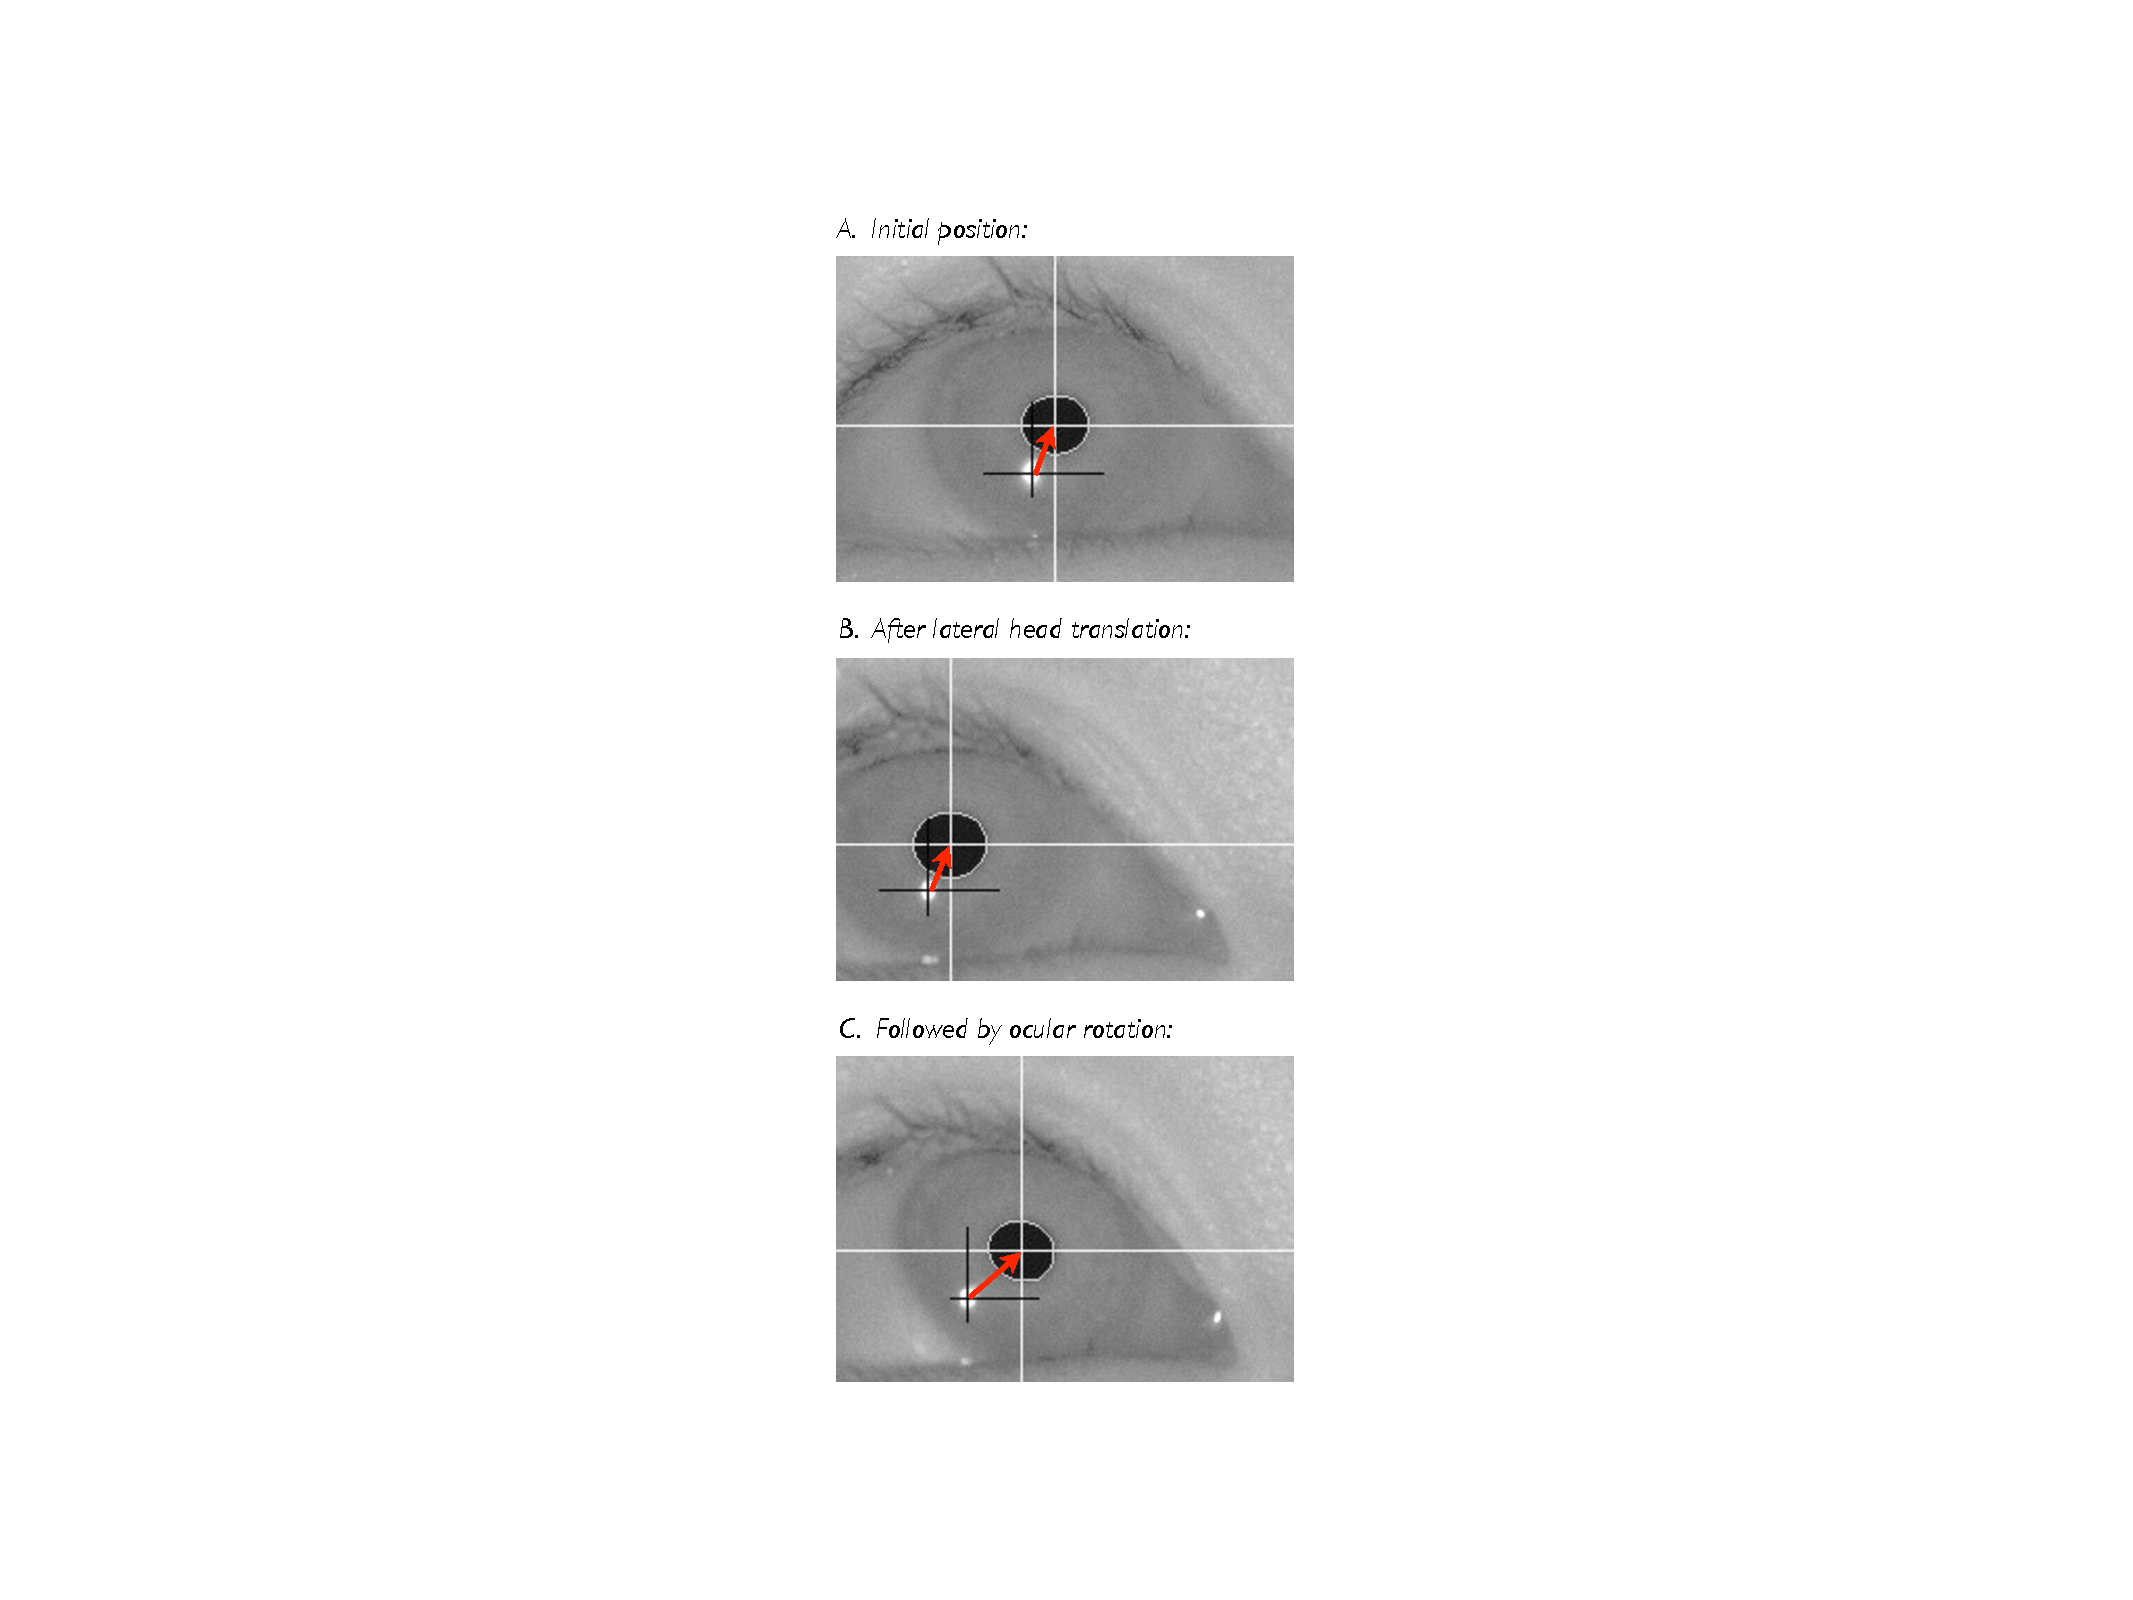
\includegraphics [width=0.25\textwidth]{Figures/Figure_1_Explanatory}
\caption{The position of the pupil within a camera image can vary due to either rotation of the eye within the head or to displacement of the head relative to the camera. Here we show how corneal reflection-stabilised pupil tracking can resolve this ambiguity. The images are individual video frames taken from the eye tracker used in this study. \textbf{\textit{(A)}} The eye tracker has identified the pupil and the first Purkinje reflection from the corneal surface, each indicated by cross-hairs. The red arrow is the vector of their relative position. \textbf{\textit{(B)}} The subject has deliberately displaced his head horizontally relative to the camera, while maintaining gaze on a centrally-located visual target. Both the pupil and the corneal reflex have shifted considerably within the video image. Their relative position, as indicated by the red arrow, remains, however, unchanged. In this case, the calibrated eye tracker would show that gaze position was stable, despite the substantial shift of the pupil within the image. \textbf{\textit{(C)}} The head remains stationary at its new location but the eye has rotated nasally within the orbit. The pupil centre and corneal reflex have moved differentially, as shown by the red arrow. By tracking the pupil-reflection relative position vector rather than the raw pupil signal, the eye tracker can yield a signal that reflects pure gaze change, without artefacts due to head motion relative to the camera.}
\label{fig:PCCR}
\end{center}
\end{figure}

% ************************
% *****    METHODS   *****
% ************************
\section{Methods}

% *****   SUBJECTS   *****
\subsection{Subjects}

Data came from an ongoing variable-endpoint longitudinal study at the New Zealand Brain Research Institute, Christchurch, New Zealand. We examined 188 patients (69\% male), with mean age 68.3 years (\textit{SD} 8.4), mean symptom duration 8.2 years (\textit{SD} 5.0), mean MDS-UPDRS part III score 33.4 (\textit{SD} 16.9) and mean Hoehn \& Yahr score 2.3 (\textit{SD} 0.7). The 66 controls (64\% male) had a mean age of 70.3 (\textit{SD} 8.5). Participants were assessed from 1-7 times (mean 2.7) over an eight year period, for a total of 491 Parkinson's and 190 control sessions. We utilised data from each visit, but the conclusions remained the same if we restricted the analysis to just one recording per person. Participants were recorded in the morning and, if prescribed, patients were on their usual anti-parkinsonian medication.

A movement disorders specialist (TJA) confirmed that patients met the UK Brain Bank criteria for idiopathic Parkinson's \citep{Hughes1992Accuracy-of-cli}. Exclusion criteria were previous history of other neurological, psychological or medical conditions, including atypical Parkinson's disease; moderate or severe head injury, stroke, major depression or learning disability; a history of cranial neurosurgery; major heart disease; diabetes requiring insulin; and alcohol abuse. All subjects gave written consent to participate in the study, which was approved by the Ethics Committee of the New Zealand Health and Disability Commission. 

% ***** APPARATUS *****
\subsection{Apparatus}
Eye movements were recorded with an iView~X Hi-Speed (SMI, Berlin), an infrared pupil and corneal reflection video tracking system. We acquired samples monocularly at 1250~Hz (usually from the left eye). Participants were seated, with forehead and chin resting upon the eye tracker column. Although participants were encouraged to keep as still as possible during recordings, the head was not physically restrained.

% ***** PROCEDURE *****
\subsection{Procedure}
Participants performed a range of oculomotor saccadic tasks in response to a jumping red square target. Only data from the first, simple visually-guided task is presented here, as it is similar to the task recorded by \cite{Gitchel2012Pervasive-ocula}. Our task has been fully described elsewhere \citep{MacAskill2012The-influence-o}, in an earlier overlapping cross-sectional sample of 163 patients and 48 controls.
In essence, the target (subtending 0.75~deg) jumped at inter-stimulus intervals ranging from 550 to 1800~ms, moving purely horizontally by pseudo-random steps of 5, 10, 15 or 20~deg leftwards or rightwards. The new target position was constrained to always remain within 15~deg of centre and served as the fixation point for the next trial. The task duration was 121~s, comprising 108 target steps.

% ***** DATA PROCESSING *****
\subsection{Data processing}
Data processing and analysis was performed in the \textit{Python} programming language (version 2.7.8) using the packages \textit{numpy} (1.9.1) and \textit{scipy} (0.14.0). Raw horizontal and vertical coordinates of the centroids of the pupil and the corneal reflection were determined within each $224 \times 160$ pixel video frame by the manufacturer's algorithm. We isolated periods of fixation by deleting sections where a saccade was present (aggressively defined as intervals in the pupil-centre signal in which the velocity exceeded 150 pixels per second, with the resulting window extended by 20 ms before and after). These parameter values were shown by visual inspection to effectively exclude saccades while retaining periods of fixation. Regions where tracking was lost (such as during blinks) were excluded.

The resulting pupil and corneal reflection signals from the fixation periods were filtered and down-sampled (decimated) to 125 Hz using a 30 point finite impulse response filter with a Hamming window to eliminate high-frequency noise. This reduced the maximum detectable frequency to 62.5 Hz, well above our expected maximum frequency of 30 Hz for any tremor of mechanical or neurogenic origins. Subtracting the decimated corneal reflection signal from the decimated pupil signal generated the reflection-corrected signal. The gradients of the pupil, reflection, and reflection-corrected signals were then calculated using central differences in the interior and first differences at the boundaries. This removed the constant offsets due to the differing gaze angles across fixations. We used principal component analysis to determine the axis of primary variability (horizontal, vertical, or oblique) in the pupil gradient data.

The power spectra of the entire decimated, differentiated, and projected pupil, reflection, and reflection-corrected signals for each subject were then determined by fast Fourier transforms, with a window size of 1024 samples and an overlap of 512 samples (equating to a moving window of 8.2 s with an overlap of 4.1 s). For each subject, a mean power spectrum across windows was produced for each of the three signals. The spectrum was then corrected for the scaling caused by differentiating the signal, and multiplied by the frequency response of a band-pass Butterworth filter (5th order, low cut-off of 1.0 Hz, high cut-off of 40 Hz) to remove the DC component. From each spectrum, the power value at the highest peak (i.e. the maximum power) was determined, along with the frequency at which it occurred.

This analysis was designed to be fully reproducible, with analysis code and raw data made open and publicly available online in an Open Science Framework repository \citep{Myall2016Investigating-o}.

% ***** STATISTICAL ANALYSIS *****
\subsection{Statistical analysis}
Our primary quantitative results (Figures \ref{fig:traces}, \ref{fig:FFT}, \ref{fig:main}) are presented without accompanying inferential statistics. The competing hypotheses were that a feature in one signal either is, or is not, abolished by subtracting another signal from it. Sample variability is not a tenable explanation for an effect of the resulting magnitude. That is, meaningful alternative explanations will be mechanistic rather than probabilistic.

In a secondary analysis, to quantify any relationships between clinical somatomotor tremor severity and eye signal oscillation power, we used a linear mixed-effects model, which could account for the repeated measures within subjects. This model (in \textit{lmer}) had the following form, relating the maximum power value for each subject's recording(s) to the MDS-UDPRS tremor sub-score from that session: 
\begin{equation}\label{eq:model}
\log_{10} (max power) \sim tremor + (1 + tremor | subject)
\end{equation}
We fitted this separately to data from each signal type (pupil, corneal reflection, or pupil--corneal reflection), as indicated by the red lines in Figure~\ref{fig:UPDRS}.

% ************************
% *****   RESULTS    *****
% ************************
\section{Results}
Principal component analysis revealed that the primary direction of any pupil signal oscillation was close to the horizontal for nearly all patients and controls. The following results are therefore based on analysis of the horizontal component of the data. Brief extracts from four representative Parkinson's recordings are shown in Figure~\ref{fig:traces}. Apparent pupil signal oscillations ranged from striking (Figure~\ref{fig:traces}A, \ref{fig:traces}B), with obvious head motion at the time of recording, to subtle (Figure~\ref{fig:traces}C, \ref{fig:traces}D). Regardless, in all four cases, the corrected signals (the difference between the raw pupil and corneal reflex signals) show no apparent oscillation. That is, pupil centre-corneal reflection subtraction is clearly effective at removing head movement artefacts.

% ***** FIGURE TRACES *****
\begin{figure*}[htbp]
\begin{center}
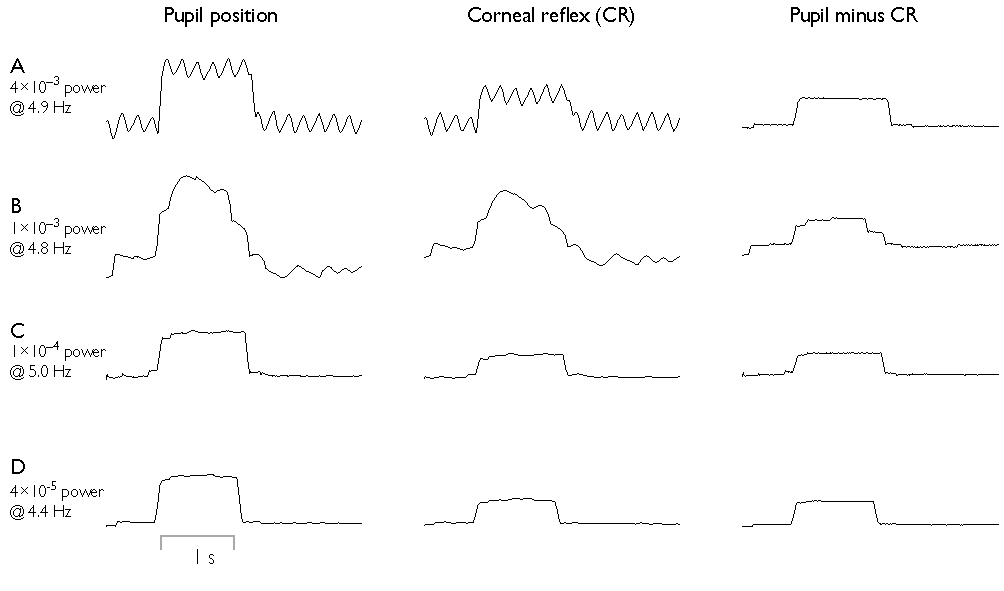
\includegraphics {Figures/Figure_2_Individual_traces}
\caption{Representative eye tracking signals from four Parkinson's participants who fell in the putative range of ``ocular tremor'' frequency in their raw pupil signal (\textasciitilde{}3 s of data as the eyes tracked a target which stepped 20 deg rightwards and then leftwards). The first column shows the raw position of the centre of the pupil within the camera image, while the second shows the position of the corneal reflection. The final column shows the difference between the two signals. Varying signal amplitudes across the subjects reflect that these are raw, uncalibrated data. \textbf{\textit{(A, B):}} These participants had upper limb tremor which was transmitted to the head, causing a major head motion artefacts in both the raw pupil and corneal reflection signals. \textbf{\textit{(C, D):}} These participants had much lower peak power in their raw signals, with any oscillation being much more subtle.
The effectiveness of simply taking the difference between the two raw signals is shown in the right-most column, in which head motion artefacts are eliminated. All four corrected signals show similarly stable gaze fixations, despite the striking range of head motion across subjects.
}
\label{fig:traces}
\end{center}
\end{figure*}

Figure \ref{fig:FFT} reveals the key finding graphically, showing the power spectrum of each recording's fixation periods, derived from the Fourier transform of each signal. There were clear peaks in the somatomotor tremor frequency range in both the raw pupil and corneal reflex signals. These peaks were common and prominent in the Parkinson's group but also occurred, albeit less commonly and at lower magnitude, in the control group. These peaks were entirely abolished in the corneal reflection-corrected data (Figure \ref{fig:FFT}, right-most column). This cancellation indicates that the peaks in the raw signals were due to a shared oscillation, which, given the principles illustrated in Figure \ref{fig:PCCR}, must have been due to head motion relative to the camera.

% ***** FIGURE FFTs *****
\begin{figure*}[htbp]
\begin{center}
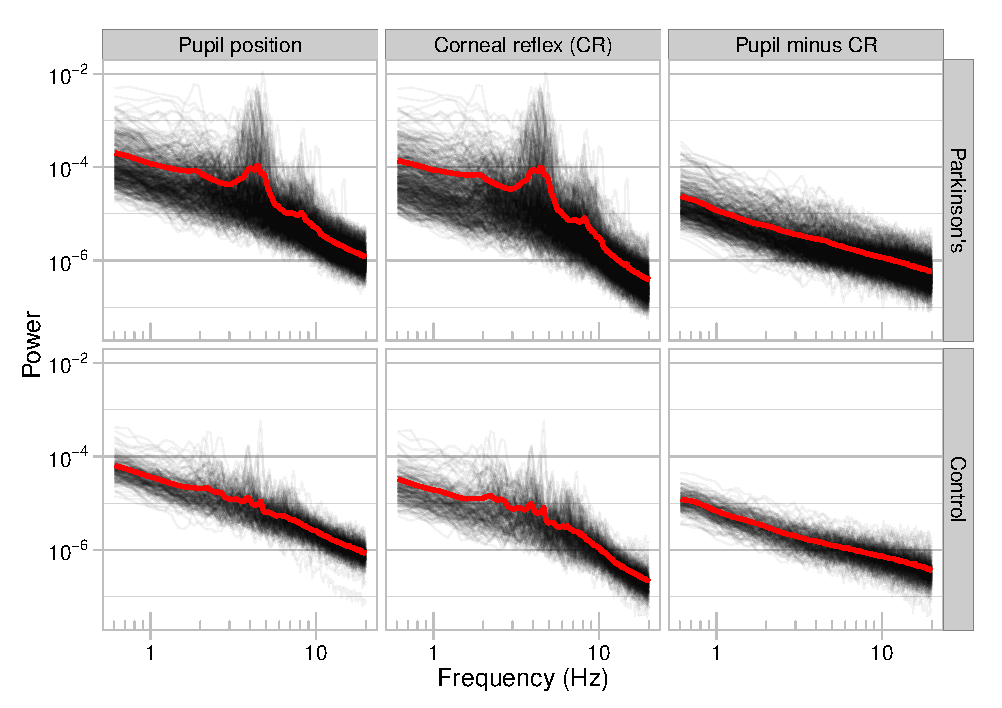
\includegraphics {Figures/Figure_3_Individual_FFTs}
\caption{For every session, we applied a fast Fourier transform (FFT) to reveal the frequency content of its pupil, corneal reflex, and pupil-minus-corneal-reflex signals (black lines). Red lines show the mean FFT of each type of signal in the Parkinson's (top panels) and Control groups (bottom panels). There is clear evidence of a peak in the vicinity of \textasciitilde4~Hz in the pupil signals from the Parkinson's group. An almost identical peak occurs in the corneal reflex signal. It is completely abolished in the signal formed by simply subtracting the corneal reflex from the pupil signal (right-most panels). This indicates that the oscillation was common to the two signals, and hence due to head motion. A similar abolition was evident in the control data, where a small number of participants also showed peaks in the somatic tremor range. We believe that the 4~Hz activity in the pupil signal is the same oscillation reported by Gitchel et al. That this is abolished when correcting with the corneal reflex signal indicates that it is an artefact of head motion relative to the camera rather than an oscillation of intrinsically ocular origin.}
\label{fig:FFT}
\end{center}
\end{figure*}

To more clearly depict individual-level data, from each of the FFTs depicted in Figure \ref{fig:FFT} we determined, for every recording from each participant, the peak power of each of their three signals (raw pupil position, corneal reflex position, and the difference between them) and the frequency at which that peak occurred (Figure \ref{fig:main}). This corresponds to the findings of \citet{Gitchel2012Pervasive-ocula}, in that the distribution of the maximum power of the pupil signal in Parkinson's participants showed a clear peak within the grey region of Figure \ref{fig:main} (representing Gitchel et al.'s reported tremor range of 5.7 $\pm$ 3 Hz). The distribution of peak frequencies across the patients in our data was, however, multimodal, showing that  oscillation in that frequency band was not universal. The distribution of frequencies was similar in the controls (see the histograms along the $x$ axes of Figure \ref{fig:main}). The distribution of oscillation power (on the $y$ axis) was clearly different, however, with controls clustering at lower values, presumably indicating the lower amplitude of any somatomotor tremor in that group.

% ***** FIGURE MAIN *****
\begin{figure*}[htbp]
\begin{center}
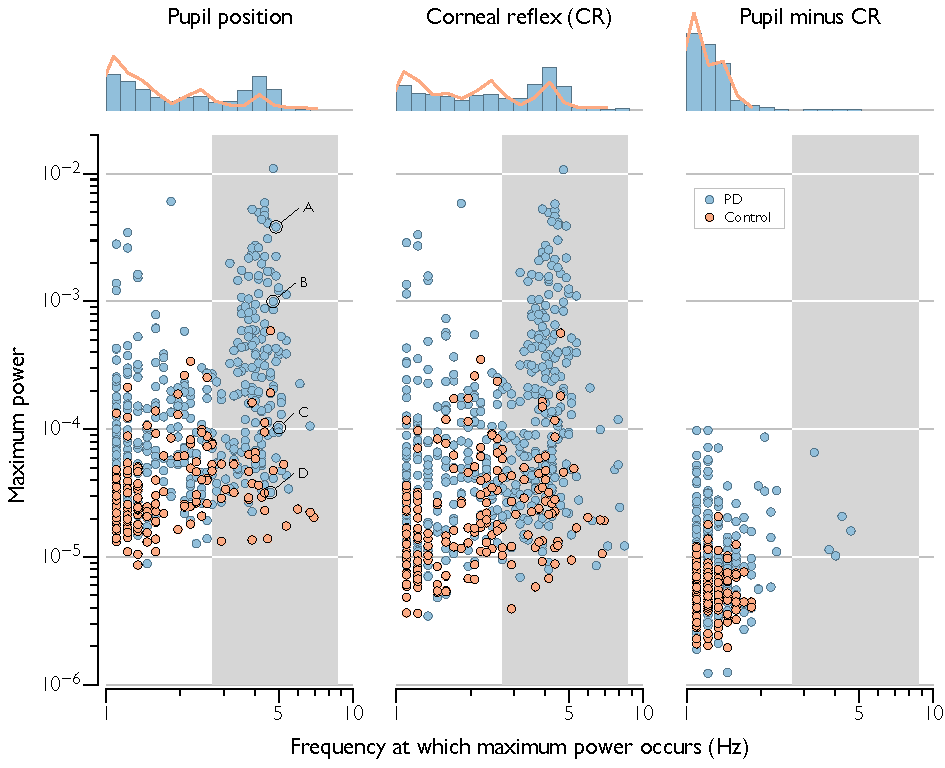
\includegraphics {Figures/Figure_4_Main_frequency_data}
\caption{For each session, a Fast Fourier Transform was applied to data from the ocular fixation periods (see Figure \ref{fig:FFT}). Points represent the peak power in each signal (left panel = raw pupil position, middle = raw corneal reflex position, right = the difference between the two) and the frequency at which it occurred. Blue points = PD, orange = Control. The labelled points \textbf{\textit{(A-D)}} correspond to the selected recordings shown in Figure \ref{fig:traces}. For reference, the grey rectangular regions represent the mean tremor frequency $\pm$ 2\textit{SD} (5.7 $\pm$ 3 Hz) reported by \cite{Gitchel2012Pervasive-ocula}. The histograms (top) reveal that one of several modes for maximum power occurs at approximately 4 Hz in the pupil and corneal reflex signals, in both the patients and controls. Although the frequency distribution ($x$ axis) was similar across the groups, the power distribution ($y$ axis) shows that the strongest oscillations were more common in PD (on re-examination, the control with the highest power value was found to have a bilateral arm tremor of that was judged to not be of extra-pyramidal origin). In the difference signal (i.e. pupil minus corneal reflex), the peak near 4 Hz was effectively abolished, with the distribution becoming dominated by what may be low frequency drift. That is, when head motion was corrected for by subtracting the corneal reflex signal from the pupil signal, the direction of gaze remained stable in space. This is strong evidence that there was no purely ocular tremor in either the Parkinson's cases or controls.}
\label{fig:main}
\end{center}
\end{figure*}

The middle panel of Figure \ref{fig:main} shows information not measured by Gitchel et al.: the peak power and oscillation frequency of the corneal reflection signal. It can be seen that its distribution in both dimensions is almost identical to the pupil data. That is, both signals appear to exhibit the same frequency and power properties. The right-most panel of Figure \ref{fig:main} shows values from the signal formed by subtracting the corneal reflection signal from the pupil signal. As in Figure \ref{fig:FFT}, any common oscillation was removed by the subtraction and we see that just five recordings had peak values which remained within the proposed tremor frequency range (the grey region), albeit at only low power.

The abolition of the putative ``tremulous'' oscillation signal following corneal reflection correction suggests strongly that it was indeed secondary to head motion. We therefore expected some relationship between the clinically-rated severity of somatomotor tremor (as assessed by the sum of the MDS-UPDRS tremor item scores) and any oscillation in the pupil and corneal reflection signals. Given the effectiveness of the corneal reflection stabilisation, we expected little to no relationship with the difference signal. Each of these predictions was supported by the data (Figure \ref{fig:UPDRS}). The models were run on log transformed data and hence their parameters correspond to the exponents on the $y$ axis of Figure \ref{fig:UPDRS}. For the pupil signal, log peak oscillation power increased linearly with increasing tremor score (slope~0.043, \textit{SE}~0.009, \textit{p}~<~0.00001). The corneal reflection signal showed a similar relationship (slope~0.046, \textit{SE}~0.010, \textit{p}~<~0.00001). The slope for the corrected pupil--corneal reflection signal (--0.004, \textit{SE}~0.004), however, was not significantly different from zero (\textit{p}~=~0.35), indicating no evidence of a relationship between tremor severity and this measure. Control subjects were not assessed with the MDS-UPDRS.

% ***** FIGURE UPDRS *****
\begin{figure*}[htbp]
\begin{center}
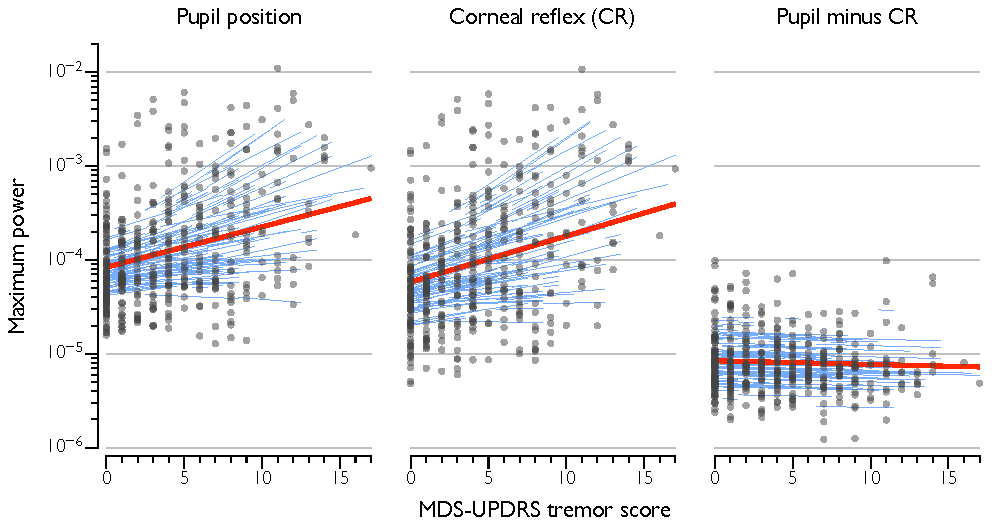
\includegraphics {Figures/Figure_5_UPDRS_correlation}
\caption{Circumstantial evidence that the apparent oscillation in ocular signals was due to somatomotor tremor. Across the 186 patients for whom at least one UPDRS assessment was available, the logarithm of the peak power of the oscillation in both the pupil and corneal reflex signals was positively related to the severity of somatomotor tremor (assessed as the sum of 10 tremor items in the MDS-UPDRS, with a maximum score of 40). No such relationship was evident in the corneal reflex-stabilised signal (rightmost panel). The linear mixed effects model (Equation \ref{eq:model}) applied to each signal accounted for the repeated assessments in many of the patients. The thick red lines show the group-level relationship between tremor and maximum signal power, while the thin blue lines depict the fits within each subject's data.
}
\label{fig:UPDRS}
\end{center}
\end{figure*}

% ************************
% *****  DISCUSSION  *****
% ************************
\section{Discussion}
We present substantive evidence that the proposed ocular diagnostic sign for Parkinson's is simply an artefact of head motion. We replicated \citet{Gitchel2012Pervasive-ocula} by showing that an oscillation was indeed often present in the raw pupil position signals of people with Parkinson's. When corneal reflection stabilisation was applied to correct for head motion, however, that apparent tremulousness was entirely abolished (Figures \ref{fig:traces}, \ref{fig:FFT}, \ref{fig:main}). Lastly, we showed that oscillatory power in the pupil and corneal reflex signals was strongly correlated with the clinical severity of somatomotor tremor. No such relationship existed in the head-motion corrected signal (Figure \ref{fig:UPDRS}). Our study was, therefore, not a failure to replicate the original finding. Rather, it is a direct refutation: we detected a pupil oscillation with similar characteristics to that described by Gitchel et al. but also demonstrated that it was due to head-camera relative motion rather than being ocular in origin.

We found the frequency distribution of the dominant oscillation to be similar between patients and controls (Figure \ref{fig:main}, $x$ axis) although the amplitudes of those oscillations were in general higher in the patients (Figure \ref{fig:main}, $y$ axis). When present, that the head-motion related oscillations in controls and patients were of similar frequencies is itself interesting. It suggests that small-amplitude somatomotor tremor, near the characteristic frequency generally ascribed to Parkinson's, is not uncommon in healthy older adults. It also indicates that video-oculography may be indirectly sensitive to signs of subtle, sub-clinical somatomotor tremor \citep{MacAskill2013Ocular-tremor-i}. Parkinson's patients themselves frequently report a sensation of ``internal tremor'', prior to the development of clinically-evident shaking \citep{Shulman1996Internal-tremor}. Although there was a strong relationship between somatomotor and ``ocular'' tremor (Figure \ref{fig:UPDRS}), there was a wide range of eye-signal oscillation power even across patients with a clinically-rated tremor score of zero. This is most likely due to the limitations of using a clinical rating scale, rather than suitable instrumented limb tremor measurement simultaneous to the eye movement recording. Parkinson's tremor can fluctuate markedly from one situation to another, depending on when the patient is feeling relaxed versus, say, experiencing performance anxiety. Part of the effect, however, may be due to the sensitivity of non-corneal reflection-stabilised video-oculography in detecting sub-clinical tremor. 

That there was evidence of tremor in some controls might be supportive of the characteristic rest tremor of Parkinson's being an amplification of a normal phenomenon. Traditionally, Parkinson's rest tremor has been viewed as an inherently pathological oscillation \citep{McAuley2000Physiological-a}. Alternatively, could it be due to abnormally increased output from an oscillatory motor control network that drives normal voluntary rhythmical movement \citep{Burkhard2002Voluntarily-sim,Schnitzler2005Normal-and-path,Schnitzler2006Physiological-a}, such as thalamo-cortical-thalamic motor circuits with a natural resonance frequency of 4-5 Hz \citep{Volkmann1996Central-motor-l}?

Could the conflict between our conclusions and those of Gitchel et al. be due to eye tracking hardware differences? Our SMI column-based eye tracker provides chin and forehead rests, with no physical restraint upon the subject. A person with head motion is therefore able to move relatively freely with respect to the camera. For the EyeLink, however, with its cameras attached to a headband, relative head-camera motion is due only to headband slippage and thus constrained to be of very small amplitude. Using the SMI system was therefore likely to be conservative with respect to disproving the ocular tremor hypothesis. With the head unrestrained relative to the camera, apparent pupil oscillation due to head motion can be of much greater amplitude than in a headband-mounted tracker. Even if our hypothesis was correct, if the corneal reflection correction technique was not highly effective, we were actually at greater risk of detecting a residual (artefactual) oscillation in the stabilised signal than if we had been using a head-mounted system with the same correction applied. One difference between our findings that might be explained by equipment differences was the dominant direction of the pupil oscillation. In our data, it was primarily horizontal (consistent with our visual observations of the eye image during recordings of people with noticeable somatomotor tremor), whereas for Gitchel et al. it was primarily vertical. This may reflect that the head is free to move relative to the world when wearing the EyeLink system, whereas with the column-mounted chin and forehead rests of the SMI, natural vertical head motion is somewhat inhibited and perhaps is more naturally expressed horizontally due to those physical constraints.

Gitchel first reported the ocular oscillation in \citeyear{Gitchel2009Oculomotor-cont}, writing that ``the hallmark feature of eye movements in Parkinson's disease is a pendular nystagmus during fixation, and all saccadic activity [is] normal.'' By 2012, Gitchel et al. argued against the phenomenon being pendular nystagmus \textit{per se} and settled on the term ``ocular tremor''. This was partly on the basis of dissimilar waveform characteristics but also because crucially, unlike nystagmus, the phase of the oscillation was not reset by saccades. \citet{Leigh2013Tremor-of-the-e} went further, noting ``probably every other form of ocular oscillation has been reported to be influenced by saccades, gaze angle, convergence, or vestibular stimuli... Lack of such influence would point to a source for PD pervasive ocular tremor outside of the ocular motor system, such as head tremor (transmitted limb tremor, in some patients).'' Based on our data, we concur with this: we reject the existence of a diagnostic ocular oscillation in Parkinson's, and regard it as an artefact of not applying corneal-reflex stabilisation to compensate for head-camera relative motion. The report by Gitchel et al. remains of value, however: oculomotor data may yet provide indirect insights into the origin of the disorder's characteristic resting somatomotor tremor and even assist prodromal diagnosis on that indirect basis.

% ************************
% **** ACKNOWLEDGMENTS ***
% ************************
\section{Acknowledgments}
The data came from a series of projects funded by the Canterbury Medical Research Foundation, Neurological Foundation of New Zealand, and New Zealand Brain Research Ltd.

Very useful comments on a preliminary version of this manuscript were made following a presentation to members of the Eye Data Quality (EDQ) Standardisation Project.

The authors declare that there is no conflict of interest regarding the
publication of this paper.

% ************************
% **** BIBLIOGRAPHY   ****
% ************************
\bibliography{ocular_tremor}

\end{document}
